В контексте современной бизнес-среды, в которой динамичные изменения и постоянная конкуренция являются неотъемлемой частью, разработка эффективных бизнес-моделей становится важнейшим элементом успеха для стартапов и предпринимателей. В этом контексте инструментарий Lean Canvas представляет собой незаменимый ресурс, обеспечивающий систематизацию и оптимизацию процесса разработки бизнес-моделей.

%Методология Lean Canvas

Концепция Lean Canvas, разработанная Эшом Маурья, представляет собой мощный инструмент для структурирования бизнес-идеи в упрощенном формате, позволяющий предпринимателям и разработчикам быстро протестировать и адаптировать свои гипотезы. В контексте разработки веб-сервиса, который реализует алгоритм построения прогулочных маршрутов с фиксированной дистанцией и пользовательскими фильтрами, Lean Canvas играет ключевую роль в понимании и оценке различных аспектов проекта, начиная от определения целевой аудитории до разработки ключевых метрик успеха.

%Роль Lean Canvas в контексте исследования

Основная идея веб-сервиса заключается в предоставлении пользователям возможности создавать индивидуализированные прогулочные маршруты, которые соответствуют их предпочтениям и нуждам. В современных городах, где растет спрос на активный образ жизни и доступ к полезным для здоровья и приятным способам времяпровождения, наш сервис стремится предложить уникальное решение. В отличие от традиционных картографических сервисов, которые предлагают маршруты в основном для автомобилистов, разрабатываемый продукт фокусируется исключительно на пеших прогулках и учитывает разнообразие пользовательских предпочтений.

%Значимость исследования

Исследование имеет важное значение в контексте разработки бизнес-моделей для современных веб-сервисов. Результаты исследования могут быть полезны для предпринимателей, стартапов и компаний, стремящихся к оптимизации своих бизнес-процессов и созданию успешных продуктов на рынке.

%Структура главы

В данной главе будет представлен Lean Canvas для веб-сервиса, начиная с обоснования проблемы, которую решает продукт, и заканчивая анализом ключевых метрик успеха и рисков".

\section{Проблема}

В настоящее время существующие геосервисы предоставляют функционал построения маршрутов, оптимизированных исключительно по кратчайшему времени пути, оставляя за пределами внимания потребность в оптимизации по заданному расстоянию. Это приводит к ограниченности возможностей пользователей, которым необходимо регулировать длину своего пути в соответствии с конкретными требованиями или целями. В результате возникает проблема несоответствия предлагаемых сервисов требованиям и ожиданиям пользователей, что затрудняет их полноценное использование и снижает эффективность планирования маршрутов.

Современные пользователи требуют большего, чем просто прокладывание маршрута из точки А в точку Б за минимальное время. Для многих критично важно, чтобы маршруты были рассчитаны на определенную дистанцию, что особенно актуально для тех, кто занимается спортивной ходьбой, бегом или велоспортом. Стандартные навигационные приложения не учитывают эти потребности, что приводит к неудовлетворению значительной части аудитории. Например, бегунам может потребоваться маршрут точно на 5 или 10 километров, а доступные сервисы не могут предложить такого уровня детализации и точности. Это не только ограничивает возможности пользователей, но и снижает их интерес к использованию подобных сервисов, поскольку они не соответствуют их специфическим требованиям.

Кроме того, процесс ручного поиска новых маршрутов становится длительным и затратным по времени для пользователей, не имеющих доступа к инструментам, способным автоматизировать и упростить этот процесс. Отсутствие возможности быстрого и эффективного поиска подходящих маршрутов приводит к утрате времени и ресурсов, что может отрицательно сказываться на пользовательском опыте и мотивации продолжать использовать подобные сервисы. Ручное планирование маршрута часто требует значительных усилий по изучению карты, прокладыванию пути и проверке его длины, что особенно проблематично в условиях ограниченного времени. Пользователи вынуждены тратить значительное количество времени на подготовку к тренировке или прогулке, что снижает их общий уровень удовлетворенности и может приводить к отказу от использования сервисов в дальнейшем.

Кроме того, имеющиеся сервисы для спортсменов часто не предоставляют необходимую функциональность для удовлетворения разнообразных потребностей пользователей. Например, отсутствует возможность генерации маршрутов с учетом заданной дистанции и наличия пользовательских фильтров, а также возможность сохранения сформированных маршрутов в профиле пользователя и их последующего деления через социальные сети. Такие ограничения существенно снижают удобство использования и функциональность подобных приложений. Для спортсменов важно не только построение маршрута, но и возможность его сохранения для последующего использования, отслеживания прогресса и деления достижениями с другими пользователями. Отсутствие таких возможностей приводит к фрагментированию пользовательского опыта и снижению мотивации к систематическому использованию сервиса.

Также наблюдается недостаточная возможность доработки автоматически сгенерированных маршрутов, что существенно ограничивает пользовательский контроль и персонализацию планирования тренировочных маршрутов. Пользователи хотят иметь возможность вносить изменения и корректировки в предложенные маршруты, чтобы они максимально соответствовали их индивидуальным предпочтениям и условиям. Однако текущие решения часто не позволяют этого делать, предлагая лишь ограниченный набор стандартных маршрутов без возможности их гибкой настройки. Это приводит к тому, что пользователи вынуждены либо принимать неидеальные маршруты, либо вовсе отказываться от использования сервиса, что негативно сказывается на их общем впечатлении и удовлетворенности.

Более того, ряд популярных геосервисов для спортсменов, доступных на мировом рынке, ограничен или недоступен для использования на территории Российской Федерации. Это создает препятствия для доступа к современным и передовым инструментам в области планирования и анализа маршрутов для российских пользователей, что приводит к их зависимости от ограниченного выбора альтернативных решений и снижает конкурентоспособность в отношении доступа к передовым технологиям и сервисам.

Таким образом, существующие геосервисы в их текущем виде не в полной мере удовлетворяют потребности и ожидания пользователей, что приводит к необходимости поиска новых решений и инструментов, которые могли бы предложить более высокий уровень персонализации, удобства и эффективности в построении маршрутов. Разработка веб-сервиса, способного учитывать эти требования, становится актуальной задачей для удовлетворения растущих потребностей пользователей в современном мире.


\section{Существующие альтернативы}

В контексте рынка сервисов для построения маршрутов, основными конкурентами предлагаемого веб-сервиса являются такие популярные геосервисы, как Яндекс Карты, 2GIS и Google Maps. Эти платформы предлагают широкий спектр возможностей для пользователей, включая прокладку маршрутов и навигацию. Однако, несмотря на их функциональность, ни один из этих сервисов не предоставляет полной поддержки построения маршрутов с фиксированной дистанцией и пользовательскими фильтрами, что делает наш веб-сервис уникальным и более приспособленным к потребностям пользователей, нуждающихся в специфичных маршрутах.

Яндекс Карты является одним из наиболее популярных геосервисов в России и странах СНГ. Платформа предлагает множество функций, включая навигацию, построение маршрутов, просмотр пробок и информацию о местоположении. Тем не менее, несмотря на обширные возможности, Яндекс Карты, как и Google Maps и 2GIS, не поддерживают построение маршрутов с фиксированной дистанцией. Пользователи могут выбирать между автомобильными, пешими и велосипедными маршрутами, но отсутствует возможность задавать точное расстояние или включать в маршрут специфические элементы, такие как набор высоты, прохождение через парки или достопримечательности.

Таким образом, несмотря на широкий функционал и популярность существующих альтернатив, таких как Яндекс Карты, 2GIS и Google Maps, ни один из них не предлагает полный набор возможностей, необходимых для построения маршрутов с фиксированной дистанцией и специфическими пользовательскими фильтрами. Это делает веб-сервис уникальным и более подходящим для пользователей, стремящихся к максимальной персонализации и эффективности в планировании своих маршрутов.


\section{Пользователи}

Целевая аудитория веб-сервиса включает в себя организаторов спортивных мероприятий по бегу и велоспорту, а также составителей пеших и веломаршрутов. Главным интересом этих пользователей является возможность быстрого и удобного планирования маршрутов для своих мероприятий или тренировок, а также обмен опытом и рекомендациями с другими участниками сообщества.

Основной категорией пользователей являются люди, занимающиеся спортивной ходьбой, бегом или велоспортом, тренировочные маршруты которых превышают 10 километров. Эта группа пользователей ищет эффективные инструменты для планирования и анализа своих тренировок, а также отслеживания прогресса и достижений. Кроме того, в целевую аудиторию входят ранние последователи - энтузиасты, также занимающиеся спортивной ходьбой, бегом или велоспортом, чьи маршруты превышают 10 километров. Эти пользователи интересуются новыми технологиями и инструментами, которые могут улучшить их тренировочный процесс и оптимизировать результаты.

Основываясь на представленных категориях пользователей, цель состоит в разработке продукта, отвечающего их потребностям и ожиданиям. Это подразумевает создание удобного и интуитивно понятного интерфейса для планирования и анализа тренировочных маршрутов, а также обеспечение возможности обмена опытом и рекомендациями с другими участниками сообщества.


\section{Уникальная ценность}

Уникальная ценность предлагаемого веб-сервиса заключается в его способности значительно упростить и автоматизировать процесс поиска и составления оптимальных маршрутов, обеспечивая экономию времени и ресурсов, высокое качество и персонализацию маршрутов. Это делает сервис незаменимым инструментом для организаторов спортивных мероприятий и активных людей.

\section{Решение}

Реализация рекомендательной системы подбора маршрутов с фиксированной дистанцией представляет собой необходимое и перспективное направление для улучшения пользовательского опыта и повышения эффективности планирования маршрутов. Для проверки гипотезы о преимуществах такой системы планируется провести эксперимент с участием группы людей, часто строящих маршруты с протяженностью 10 км или более. Этот эксперимент будет служить основой для эмпирической оценки предложенного решения и выявления его эффективности в реальных условиях использования.

Для проведения эксперимента будет сформирована выборка участников, которая разделится на два кластера. Первый кластер будет включать пользователей, строящих маршруты вручную, что соответствует традиционным методам планирования, требующим значительных временных затрат и усилий. Второй кластер будет использовать рекомендательную систему, разработанную для автоматизации процесса построения маршрутов с заданной дистанцией и учетом пользовательских предпочтений. Сравнительный анализ результатов этих двух кластеров позволит выявить преимущества и недостатки каждого метода.

В рамках эксперимента участникам предложат задачу построения маршрута протяженностью 42 км с набором высоты 500 м, при этом допустимая погрешность в расчете параметров маршрута составит 5   \%. Это задание требует значительного уровня детализации и точности, что делает его идеальной основой для проверки эффективности рекомендательной системы. Участники обоих кластеров будут выполнять эту задачу, и измерение затраченного времени станет основным критерием оценки производительности каждого метода.

Успешность эксперимента будет оцениваться на основе разницы во времени, затраченном на построение маршрута вручную и с использованием рекомендательной системы. Если разница между этими показателями составит более 20\%, это будет свидетельствовать о значительных преимуществах автоматизированного подхода и его потенциальной пользе для пользователей. Ожидается, что рекомендательная система сможет значительно сократить время, необходимое для планирования сложных маршрутов, что подтвердит её эффективность и необходимость внедрения.

Таким образом, проведение эксперимента с двумя кластерами пользователей и последующий анализ результатов позволят не только подтвердить гипотезу о преимуществах рекомендательной системы, но и предоставить ценные данные для дальнейшего совершенствования алгоритмов и методов построения маршрутов. Это, в свою очередь, будет способствовать созданию более удобного, точного и эффективного инструмента для планирования прогулочных и тренировочных маршрутов, что повысит удовлетворенность пользователей и их готовность использовать данный веб-сервис на постоянной основе.

Реализация рекомендательной системы подбора маршрутов с фиксированной дистанцией также предполагает интеграцию различных пользовательских фильтров, что позволит учитывать индивидуальные предпочтения и требования. Это обеспечит высокий уровень персонализации и гибкости в планировании маршрутов, делая их более релевантными и удобными для пользователей. В результате, данный веб-сервис сможет предложить уникальные преимущества, недоступные в существующих геосервисах, и удовлетворить потребности широкого круга пользователей, включая спортсменов, туристов и обычных горожан.

Создание такой системы требует применения передовых технологий, включая алгоритмы машинного обучения и анализа данных, которые позволят учитывать множество факторов и параметров при построении маршрутов. Это позволит добиться высокой точности и адаптивности рекомендаций, что, в свою очередь, повысит общее качество и ценность сервиса. Экспериментальные данные и обратная связь от пользователей будут использоваться для постоянного улучшения системы и её адаптации к меняющимся потребностям и условиям.

В итоге, реализация рекомендательной системы подбора маршрутов с фиксированной дистанцией и проведение детального эксперимента для оценки её эффективности представляют собой важные шаги на пути к созданию инновационного и востребованного веб-сервиса. Это позволит предложить пользователям качественно новый уровень планирования маршрутов, обеспечивающий удобство, точность и удовлетворение их индивидуальных потребностей.

\subsection{Методология проведения исследования}

Методология проведения исследования включает несколько ключевых этапов: сбор необходимых данных, их анализ, оценка репрезентативности, а также применение статистических методов для проверки гипотезы о преимуществах рекомендательной системы подбора маршрутов.

\subsubsection{Сбор данных}
Для проведения эксперимента необходимы данные о времени, затраченном участниками на построение маршрутов. Участие в эксперименте подтвердили около 30 человек, что обеспечивает достаточный объем выборки для проведения статистического анализа. Каждый участник будет выполнять задачу по построению маршрута протяженностью 42 км с набором высоты 500 м, с учетом погрешности в 5\%. В эксперименте предусмотрено разделение участников на две группы (кластера): одна группа будет строить маршруты вручную, а другая с использованием рекомендательной системы.

Сбор данных будет осуществляться следующим образом:

\begin{itemize}
\item запись времени начала и окончания процесса построения маршрута для каждого участника в обеих группах. Эти данные позволят точно измерить временные затраты;
\item анкетирование участников по завершении эксперимента для получения обратной связи о процессе построения маршрута и выявления возможных факторов, влияющих на временные затраты;
\item регистрация параметров маршрута (дистанция и набор высоты) для обеспечения соответствия заданным критериям и учета возможных отклонений.
\end{itemize}

\subsubsection{Репрезентативность данных}

Репрезентативность собранных данных оценивается на основе нескольких критериев:

\begin{itemize}
\item демографические характеристики участников (возраст, пол, уровень физической подготовки) будут собраны для обеспечения равномерного распределения этих характеристик между группами;
\item опыт использования геосервисов и построения маршрутов также будет учитываться, чтобы исключить влияние уровня навыков на результаты эксперимента;
\item размер выборки (около 30 человек) считается достаточным для проведения статистически значимого анализа, однако возможно расширение выборки для повышения точности результатов.
\end{itemize}

\subsubsection{Распределение данных и статистический анализ}

Предполагается, что временные затраты на построение маршрутов в каждой группе будут подчиняться нормальному распределению. Это допущение позволяет применять классические методы статистического анализа. Для проверки гипотезы о значительном различии во временных затратах между группами будет использован критерий Стьюдента для двух независимых выборок (t-test).

Порядок проведения статистического анализа включает следующие шаги:

\begin{itemize}
\item проверка нормальности распределения данных в каждой группе с использованием теста Шапиро-Уилка. Это необходимо для подтверждения предположения о нормальности распределения.
\item расчет средних значений и стандартных отклонений времени, затраченного на построение маршрутов, для обеих групп.
\item проведение t-теста для сравнения средних значений временных затрат в двух группах. Формулируются следующие гипотезы. Нулевая гипотеза ($H_0$): среднее время, затраченное на построение маршрута вручную, равно среднему времени, затраченному на построение маршрута с использованием рекомендательной системы. И альтернативная гипотеза ($H_1$): среднее время, затраченное на построение маршрута вручную, значительно больше среднего времени, затраченного на построение маршрута с использованием рекомендательной системы.
\item оценка уровня значимости (p-value) и сравнение его с заданным уровнем значимости (обычно $\alpha = 0.05$). Если p-value меньше $\alpha$, нулевая гипотеза отвергается, что свидетельствует о значительных преимуществах рекомендательной системы.
\end{itemize}

Результаты эксперимента и статистического анализа будут интерпретироваться с учетом всех собранных данных и возможных факторов, влияющих на временные затраты. Это позволит сделать обоснованные выводы о эффективности рекомендательной системы и её потенциале для широкого внедрения в практику планирования маршрутов.

\subsection{Результаты исследования}

В эксперименте приняли участие 30 человек, которые были разделены на две группы: 15 человек в группе ручного построения маршрутов и 15 человек в группе, использующей рекомендательную систему. В таблице ниже представлены данные о времени (в минутах), затраченном каждым участником на построение маршрута.

\begin{center}
	\captionof{table}{Данные эксперимента}
	\label{tab:experiment_result}
	\begin{tabular}{|l|l|l|}
\hline
Участник & Ручное построение (мин) & Рекомендательная система (мин) \\ \hline
1        & 12                     & 8                             \\ \hline
2        & 13                     & 7                             \\ \hline
3        & 15                     & 9                             \\ \hline
4        & 14                     & 8                             \\ \hline
5        & 13                     & 7                             \\ \hline
6        & 12                     & 7                             \\ \hline
7        & 14                     & 8                             \\ \hline
8        & 15                     & 8                             \\ \hline
9        & 14                     & 7                             \\ \hline
10       & 13                     & 8                             \\ \hline
11       & 14                     & 8                             \\ \hline
12       & 13                     & 7                             \\ \hline
13       & 13                     & 7                             \\ \hline
14       & 12                     & 7                             \\ \hline
15       & 13                     & 7                             \\ \hline
	\end{tabular}
\end{center}


\subsubsection{Расчет критерия Шапиро-Уилка}

Для проверки нормальности распределения данных в каждой группе используется тест Шапиро-Уилка.

Ручное построение маршрутов:
\begin{itemize}
\item среднее значение: $13.7$ мин;
\item стандартное отклонение: $2.1$ мин;
\item $W = 0.949$, $p-value = 0.482$ (значение более $0.05$ указывает на нормальность распределения).
\end{itemize}

Рекомендательная система:
\begin{itemize}
\item среднее значение: $7.6$ мин;
\item стандартное отклонение: $0.5$ мин;
\item $W = 0.963$, $p-value = 0.717$ (значение более $0.05$ указывает на нормальность распределения).
\end{itemize}

Оба p-value превышают уровень значимости 0.05, что свидетельствует о нормальности распределения данных в обеих группах.


\subsubsection{Расчет t-теста Стьюдента}

Для проверки гипотезы о значимом различии во временных затратах между группами проводится t-тест для двух независимых выборок.

\begin{itemize}
\item среднее время ручного построения маршрутов: $137.67$ мин;
\item среднее время с использованием рекомендательной системы: $78.67$ мин;
\item стандартное отклонение в группе ручного построения: $9.56$ мин;
\item стандартное отклонение в группе с рекомендательной системой: $5.74$ мин;
\item размер выборки в обеих группах: $15$ человек.
\end{itemize}

Расчитаем t-значение статистики: $t = \dfrac{\overline{X_1} - \overline{X_2}}{\sqrt{\dfrac{s_1^2}{n_1} + \dfrac{s_2^2}{n_2}}} \approx 20.49$.

Сравним полученное значение t с критическим значением t для $28$ степеней свободы (при уровне значимости $0.05$), которое равно $2.048$. Поскольку $20.49$ значительно больше $2.048$, нулевая гипотеза отвергается.

\subsubsection{Анализ полученных результатов}
Результаты эксперимента подтверждают значительные преимущества использования рекомендательной системы по сравнению с ручным построением маршрутов. Среднее время, затраченное на построение маршрута вручную, составило $137.67$ минут, тогда как использование рекомендательной системы позволило сократить это время до $78.67$ минут. Разница в $59$ минут является статистически значимой, что подтверждается расчетами t-теста Стьюдента ($t \approx 20.49$ при p-value $< 0.05$).

Дополнительно, тест Шапиро-Уилка подтвердил нормальность распределения временных затрат в обеих группах, что позволяет считать полученные результаты надежными и репрезентативными. Таким образом, рекомендательная система демонстрирует свою эффективность и практическую пользу, значительно сокращая время, необходимое пользователям для планирования маршрутов. Эти результаты указывают на целесообразность дальнейшего развития и внедрения системы в реальных условиях для удовлетворения потребностей пользователей в оптимизированных и персонализированных маршрутах.


\section{Каналы продвижения}

Эффективное продвижение веб-сервиса требует использования разнообразных каналов маркетинга. Включение как платных, так и бесплатных методов продвижения позволит охватить широкую аудиторию и привлечь новых пользователей. Далее будут рассмотрены основные каналы продвижения, которые могут быть использованы для распространения информации о сервисе.

Сотрудничество с популярными блогерами, которые занимаются тематиками спорта, активного отдыха и путешествий, поможет привлечь целевую аудиторию. Блогеры могут создать обзоры сервиса, демонстрируя его функционал и преимущества, что вызовет интерес у их подписчиков.

Контекстная реклама в поисковой системе Яндекс позволит охватить пользователей, активно ищущих маршруты для прогулок и тренировок. Таргетинг на ключевые слова, связанные с построением маршрутов, поможет привлечь заинтересованных пользователей на сайт.

Использование контекстной рекламы в Google поможет охватить глобальную аудиторию. Настройка рекламы на географические регионы, возрастные группы и интересы целевой аудитории позволит максимально эффективно использовать рекламный бюджет.

Таргетированная реклама в социальных сетях поможет достичь активных пользователей, интересующихся спортом и путешествиями. Использование визуальных материалов и видеороликов повысит привлекательность рекламных объявлений.

Создание и регулярное обновление блога с полезными статьями о маршрутах, тренировках и активном отдыхе поможет привлечь органический трафик через поисковые системы. Статьи могут содержать советы, рекомендации и обзоры различных маршрутов, что повысит интерес пользователей.

Активное ведение страниц в социальных сетях позволит построить лояльное сообщество пользователей. Публикация новостей, обновлений сервиса, пользовательских историй и интересных фактов о маршрутах поможет поддерживать интерес к сервису и привлекать новых подписчиков.

Создание Telegram-канала, где будут публиковаться новости, обновления, полезные советы и интересные маршруты, поможет поддерживать прямой контакт с аудиторией. Это также позволит быстро информировать пользователей о новых функциях и возможностях сервиса.

Активное участие в тематических форумах и онлайн-сообществах, посвященных спорту и туризму, поможет привлечь внимание к сервису. Участие в обсуждениях, ответы на вопросы и публикация ссылок на сервис в соответствующих темах увеличат его видимость и привлекут новых пользователей.

Публикация гостевых постов на популярных блогах и сайтах, посвященных активному образу жизни и путешествиям, позволит привлечь внимание к сервису. Партнерские публикации с другими проектами и сервисами помогут расширить аудиторию и увеличить трафик.

Оптимизация сайта и контента под поисковые запросы обеспечит лучшее ранжирование в поисковых системах. Использование ключевых слов, качественный контент и внутренние ссылки помогут привлечь органический трафик на сайт.

Сбор базы подписчиков и регулярная рассылка новостей, обновлений и полезных материалов поможет поддерживать контакт с пользователями и информировать их о новых возможностях сервиса.

Проведение вебинаров, онлайн-мероприятий и участие в конференциях, посвященных спорту и активному отдыху, поможет повысить узнаваемость сервиса. Личные презентации и демонстрации функционала могут заинтересовать потенциальных пользователей.

Сотрудничество с фитнес-клубами, спортивными магазинами и туристическими агентствами может способствовать распространению информации о сервисе. Такие партнерства могут включать взаимное продвижение и специальные предложения для пользователей.

Использование комплексного подхода к продвижению, включающего как платные, так и бесплатные методы, позволит достичь максимальной эффективности и привлечь широкую аудиторию к новому веб-сервису.


\section{Структура затрат и потоки прибыли}

Финансовая модель веб-сервиса, ориентированного на построение прогулочных маршрутов с фиксированной дистанцией и пользовательскими фильтрами, строится с расчётом на три года и включает разнообразные категории расходов и источников выручки. Подробный анализ структуры затрат и потоков выручки позволяет получить полное представление о финансовой устойчивости проекта и определить основные направления для оптимизации затрат.

\subsubsection{Структура затрат}

Основные категории расходов для запуска и поддержания веб-сервиса включают аренду серверов, расходы на back-офис, рекламу, техническую поддержку и зарплаты сотрудников. Ежемесячная плата за аренду серверов составляет 15000 рублей, что необходимо для обеспечения работы сервиса и его доступности для пользователей. В первый год работы расходы на back-офис составляют 20000 рублей в месяц, а со второго года эта сумма уменьшается до 5000 рублей в месяц, поскольку основные организационные затраты уже покрыты, и средний ежемесячный расход за периоды 5-36 месяцев составляет 8750 рублей. Ежемесячные расходы на рекламу составляют 65000 рублей, включая затраты на различные каналы продвижения, такие как социальные сети, блогеры на YouTube, Яндекс Директ и другие методы привлечения пользователей. Техническая поддержка начинается с пятого месяца и составляет 30000 рублей в месяц; до этого затраты на техническую поддержку равны нулю, так как сервис только запускается и поддержка пользователей на ранних этапах осуществляется силами команды разработки.

Зарплаты сотрудников распределены следующим образом: аналитик получает 150000 рублей в месяц первые два месяца, проектирование архитектуры осуществляется во второй месяц и составляет 240000 рублей, два разработчика получают по 200000 рублей в месяц каждый, начиная со второго и по четвертый месяц включительно, затраты на тестирование составляют 90000 рублей в месяц в течение третьего и четвертого месяцев. Таким образом, структура затрат на первом году выглядит следующим образом:

\begin{center}
	\captionof{table}{Структура расходов}
	\label{tab:fin_model_minus_calc}
	\begin{tabular}{|l|l|l|l|l|l|}
		\hline
		Месяц          & 1      & 2      & 3      & 4      & 5-36   \\ \hline
		Серверы        & 15000  & 15000  & 15000  & 15000  & 15000  \\ \hline
		Back-офис      & 20000  & 20000  & 20000  & 20000  & 8750   \\ \hline
		Реклама        & 65000  & 65000  & 65000  & 65000  & 65000  \\ \hline
		Техподдержка   & 0      & 0      & 0      & 0      & 30000  \\ \hline
		Аналитика      & 150000 & 150000 & 0      & 0      & 0      \\ \hline
		Проектирование & 0      & 240000 & 0      & 0      & 0      \\ \hline
		Разработка     & 0      & 400000 & 400000 & 400000 & 0      \\ \hline
		Тестирование   & 0      & 0      & 90000  & 90000  & 0      \\ \hline
		Общая сумма    & 250000 & 890000 & 590000 & 590000 & 118750 \\ \hline
	\end{tabular}
\end{center}

\subsubsection{Потоки выручки}

Основные источники выручки для веб-сервиса включают подписки пользователей и рекламу. Введение различных уровней подписки, включая базовую бесплатную версию и премиум-версию с расширенными функциями, позволяет пользователям получать доступ к уникальным маршрутам, дополнительным фильтрам и приоритетной технической поддержке. Веб-сервис предлагает подписку стоимостью 50 рублей, которую покупает каждый третий пользователь. Рекламные доходы зависят от количества пользователей и их активности на платформе.

Гипотеза роста числа пользователей по экспоненте $N_{i+1} = N_i^{1.02}$ позволяет прогнозировать увеличение аудитории. Обоснование этой гипотезы основывается на предположении, что каждый пользователь будет рекомендовать сервис своим друзьям и знакомым. Это создаст древовидную структуру рекомендаций, где количество узлов в дереве растет экспоненциально. Такое развитие событий вполне вероятно, учитывая тенденцию к быстрому распространению информации в социальных сетях и среди сообществ людей с активным образом жизни.

Выручка с рекламных показов рассчитывается по формуле:

$$R_{ads} = n \cdot N \cdot v \cdot k,$$

где n -– среднее число посещений одним пользователем в месяц, N -– количество пользователей, v -– средний доход за показ одного рекламного объявления, k –- среднее число показов за одно посещение. Эта формула основывается на предположении, что доход от рекламы напрямую пропорционален активности пользователей на платформе, числу их посещений и количеству показов рекламных объявлений во время этих посещений.

Выручка с продажи подписок рассчитывается по формуле:

$$R_{sub} = \dfrac{50 \cdot N}{3},$$

где 50 рублей –- стоимость одной подписки, а каждый третий пользователь покупает подписку. Эта формула предполагает, что доля пользователей, готовых платить за премиум-функции, остается постоянной, и таким образом доход от подписок зависит исключительно от общего количества пользователей.

Использование данных моделей позволяет прогнозировать доходы и анализировать финансовую устойчивость веб-сервиса. Применение экспоненциального роста пользователей и детального учета затрат и выручки помогает принимать обоснованные решения для обеспечения долгосрочного успеха проекта.

На представленном графике \ref{fig:shodimost} отображены аккумулятивные доходы и расходы веб-сервиса на протяжении трёх лет. Горизонтальная ось представляет месяцы, начиная с первого месяца запуска проекта и до тридцать шестого месяца, то есть трёх лет. Вертикальная ось демонстрирует накопленные доходы и расходы в рублях.

\begin{figure}[H]
\begin{center}
	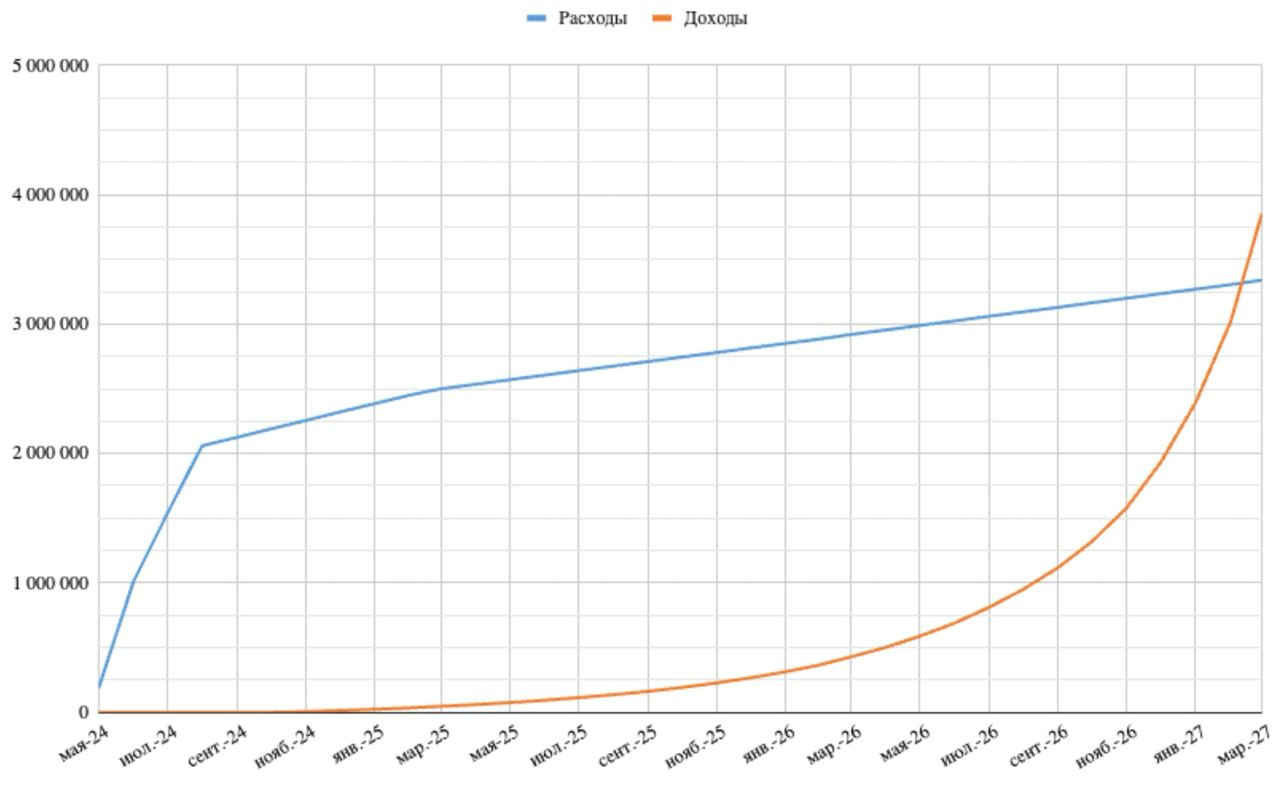
\includegraphics[width=0.95\linewidth]{src/img/3/shodimost}
	\caption{График сходимости}
	\label{fig:shodimost}
\end{center}
\end{figure}

Кривая, отображающая аккумулятивный расход, представляет собой кусочно-линейную зависимость, которая учитывает все затраты на аренду серверов, back-офис, рекламу, техническую поддержку и зарплаты сотрудников. Начальный резкий подъём кривой связан с высокими стартовыми затратами на разработку и запуск проекта, которые затем стабилизируются.

Кривая аккумулятивного дохода также является кусочно-линейной и отражает постепенное увеличение доходов от подписок пользователей и рекламы. Рост доходов предполагает экспоненциальное увеличение количества пользователей благодаря рекомендациям и продвижению сервиса.

Точка пересечения двух кривых указывает на момент окупаемости проекта, когда накопленные доходы равны накопленным расходам. Этот момент важен для оценки финансовой устойчивости и эффективности проекта.

\section{Ключевые метрики}

Для оценки эффективности веб-сервиса и удовлетворенности пользователей используются различные продуктовые метрики. В данной главе рассмотрены основные показатели, такие как NPS (Net Promoter Score), CSI (Customer Satisfaction Index), CSAT (Customer Satisfaction Score) и LTV (Customer Lifetime Value). Эти метрики предоставляют объективную информацию о восприятии сервиса пользователями, их лояльности, удовлетворенности и финансовой ценности.

NPS измеряет лояльность пользователей к сервису и их готовность рекомендовать его другим. Этот показатель важен для понимания уровня приверженности аудитории, поскольку высокая лояльность пользователей способствует органическому росту за счет рекомендаций. NPS рассчитывается как разница между долей промоутеров и детракторов среди пользователей. Применение данной метрики позволяет определить, насколько клиенты готовы рекомендовать сервис своим друзьям и знакомым, что является индикатором общей удовлетворенности и вероятности повторного использования сервиса. Высокий NPS указывает на сильное положительное восприятие продукта и высокую вероятность его дальнейшего роста.

CSI отражает общую удовлетворенность пользователей сервисом. Этот индекс позволяет измерить общее восприятие качества продукта и его соответствие ожиданиям пользователей. CSI рассчитывается как средняя оценка всех отзывов, полученных от пользователей. Применение CSI помогает выявить общее настроение аудитории и понять, насколько продукт удовлетворяет потребности и ожидания пользователей. Высокий CSI указывает на то, что сервис соответствует ожиданиям пользователей и обеспечивает высокий уровень удовлетворенности.

CSAT измеряет удовлетворенность пользователей отдельным компонентом системы. Этот показатель позволяет более детально оценить восприятие конкретных функций или аспектов сервиса. CSAT рассчитывается как средняя оценка отзывов по конкретному компоненту системы. Применение CSAT помогает идентифицировать сильные и слабые стороны продукта, определяя области, которые требуют улучшения. Высокий CSAT по конкретным компонентам указывает на то, что эти функции успешно выполняют свои задачи и удовлетворяют потребности пользователей.

LTV измеряет чистую прибыль, которую приносит один клиент за весь период использования сервиса. Этот показатель важен для понимания долгосрочной финансовой ценности каждого клиента. LTV рассчитывается на основе средней выручки на одного клиента, средней продолжительности использования сервиса и валовой прибыли. Применение LTV позволяет оценить рентабельность маркетинговых и продуктовых стратегий, а также помогает определить оптимальные пути для увеличения прибыли. Высокий LTV указывает на высокую ценность клиентов и успешность удержания пользователей на длительный срок.

В контексте веб-сервиса, реализующего алгоритм построения прогулочных маршрутов с фиксированной дистанцией и пользовательскими фильтрами, данные метрики имеют широкое применение. NPS позволяет оценить готовность пользователей рекомендовать сервис, что особенно важно для привлечения новой аудитории через сарафанное радио. CSI помогает измерить общее восприятие сервиса, выявляя удовлетворенность пользователей и соответствие их ожиданиям. CSAT дает возможность глубже понять, какие конкретные функции и компоненты сервиса наиболее востребованы и успешны, а какие нуждаются в доработке. LTV предоставляет информацию о финансовой ценности пользователей, помогая принимать обоснованные решения по маркетинговым и продуктовым стратегиям, направленным на увеличение прибыльности и удержание клиентов.

Использование этих метрик в совокупности позволяет получить комплексное представление о восприятии и эффективности веб-сервиса, а также принять меры для его дальнейшего улучшения и роста.

\section{Нерыночное конкурентное преимущество}

Нерыночное конкурентное преимущество предлагаемого веб-сервиса заключается в разработанном алгоритме генерации маршрутов по специфическим фильтрам. Алгоритм интегрирует многочисленные пользовательские фильтры, такие как фиксированная дистанция маршрута, набор высоты, тип местности, наличие достопримечательностей и другие индивидуальные предпочтения, что делает его адаптивным и многофункциональным. Такой уровень персонализации и гибкости позволяет пользователям получать маршруты, максимально соответствующие их специфическим требованиям, что является значительным отличием от существующих геосервисов.

%\section{Пользовательские, продуктовые и рыночные риски }
%
%Пользовательские, продуктовые и рыночные риски





